\documentclass[a4pape, 11pt, english]{article}
\usepackage[margin=1in,footskip=0.25in]{geometry}
\usepackage{graphicx}
\usepackage[numbers]{natbib}
% Used https://tex.stackexchange.com/questions/420588/numbered-citations-in-latex for citation numbes
\usepackage{array}
\usepackage{booktabs}
\usepackage{longtable}

\usepackage[hyphens]{url} % To wrap urls on multiple lines: https://tex.stackexchange.com/questions/115690/urls-in-bibliography-latex-not-breaking-line-as-expected

\title{Appendix}
\author{Thomas Fishwick}

\begin{document}
%\maketitle
\begin{center}
\huge
Appendix
\end{center}

\section{Glossary}
\begin{itemize}
	\item Bagging – using sampling with replacement from the data to create artificial training data (bootstrap samples)
	\item Bayesian Optimisation – a function used to run through an array of different hyperparameters for a machine learning model
	\item BFGS - (Broyden-Fletcher-Goldfarb-Shanno quasi-Newton algorithm) a second order derivative used to help optimise linear regression.\citep{brownlee_gentle_2021} (paraphrased)
	\item Decision Tree Regression – splits the data into distinct regions with the region’s mean being the response to a prediction \citep{james_gareth_introduction_2021} (paraphrased)
	\item Features - The independent variables used to predict something in Regression
	\item Hyperparameter – a parameter of the machine learning model (so named as machine learning models are used to find the parameters of a model)
	\item Labels - the target/y value in Regression
	\item Lasso Regression – Least Absolute Shrinkage and Selection Operator. Tries to eliminate as many features as possible when performing the regression to have as sparse a model as possible \citep{stephanie_lasso_2015}
	\item Linear Regression: an algorithm which attempts to fit an equation of the form $Y = wX + c$ to the data so that its error to the true value is minimised as far as possible
	\item Normalised: the data is shifted so that its mean is zero and rescaled to move its standard deviation to 1. We are excluding the zero/one categorical columns from this, as it doesn’t make sense to include them.
	\item Random Forest Regression – a collection of decision tree regressors (hence the forest) that behaves as a single model as the average prediction is returned from the collection of decision tree results. Each individual tree is trained using \textit{“bagging and random features”} \citep{schapire_robert_random_2001}. A random subset of features is given to each tree.
	\item Ridge Regression – can create a parsimonious model (small and simple model) where the number of features is greater than the number of rows. \textit{“Adds just enough bias to make the estimates reasonably reliable”} \citep{stephanie_ridge_2017} (paraphrased and directly quoted) 
\end{itemize}

\section{Intermediate results}
\begin{longtable}{m{3.4cm}m{6.6cm}m{1.5cm}m{1.5cm}m{1.5cm}}
\toprule
Type & Hyperparameters & RMSE & MAE & Accuracy (1-NMSE) \\
\midrule
Linear Regression & Default (columns: model, year, mileage, fuel type, MPG, engine size) & 4782.14 & 3602.55 & -0.04 \\
\addlinespace
\hline
Linear Regression & Default (columns: model, year, mileage, fuel type, MPG, engine size), Normalised & 2427.54 & 1717.89 & 0.73 \\
\addlinespace
\hline
Linear Regression & Lambda', 0.0002972, 'Learner', 'leastsquares', 'Regularization', 'ridge', 'Solver', 'bfgs' (columns: model, year, mileage, fuel type, MPG, engine size), Normalised & 1828.18 & 1346.7 & 0.85 \\
\addlinespace
\hline
Linear Regression & Lambda', 0.0002972, 'Learner', 'leastsquares', 'Regularization', 'ridge', 'Solver', 'bfgs' (columns: model, year, mileage, fuel type, MPG, engine size), Normalised, with validation data & 1837.15 & 1350.96 & 0.85 \\
\addlinespace
\hline
Linear Regression & Lambda', 0.000010015, 'Learner', 'leastsquares', 'Regularization', 'ridge', 'Solver', 'bfgs' (columns: model, year, mileage, fuel type, MPG, engine size), Normalised, validation & 1859.48 & 1358.33 & 0.84 \\
\addlinespace
\hline
Linear Regression & Lambda', 0.000010015, 'Learner', 'leastsquares', 'Regularization', 'ridge', 'Solver', 'bfgs' (columns: model, year, mileage, fuel type, MPG, engine size), Normalised & 1826.26 & 1347.21 & 0.85 \\
\addlinespace
\hline
Linear Regression & Lambda', 0.000010015, 'Learner', 'leastsquares', 'Regularization', 'ridge', 'Solver', 'bfgs', 'Kfold', 5 (columns: model, year, mileage, fuel type, MPG, engine size), Normalised (1st model) & 1818.02 & 1344.83 & 0.85 \\
\addlinespace
\hline
Random Forest & Default (columns: model, year, mileage, fuel type, MPG, engine size) & 1279.66 & 889.33 & 0.93 \\
\addlinespace
\hline
Random Forest (technically boosted forest) & MinLeafSize, 31, Method, LSBoost, NumLearningCycles, 193, LearnRate 0.38119. (columns: model, year, mileage, fuel type, MPG, engine size). & 1185.69 & 837.56 & 0.94 \\
\addlinespace
\hline
Random Forest & MinLeafSize, 31, Method, Bag, NumLearningCycles, 193, (columns: model, year, mileage, fuel type, MPG, engine size). & 1398.75 & 968.24 & 0.91 \\
\addlinespace
\hline
Random Forest & MinLeafSize, 1, Method, Bag, NumLearningCycles, 499, (columns: model, year, mileage, fuel type, MPG, engine size). & 1175.02 & 838.02 & 0.94 \\
\addlinespace
\hline
Random Forest & MinLeafSize, 1, Method, Bag, NumLearningCycles, 450, (columns: model, year, mileage, fuel type, MPG, engine size). & 1175.03 & 838.63 & 0.94 \\
\addlinespace
\hline
Random Forest & MinLeafSize, 1, Method, Bag, NumLearningCycles, 50, (columns: model, year, mileage, fuel type, MPG, engine size). & 1178.42 & 839.35 & 0.94 \\
\addlinespace
\hline
Random Forest & MinLeafSize, 1, Method, Bag, NumLearningCycles, 500, (columns: model, year, mileage, fuel type, MPG, engine size). & 1174.68 & 838.28 & 0.94 \\
\addlinespace
\hline
Random Forest & MinLeafSize, 1, Method, Bag, NumLearningCycles, 499, (columns: model, year, mileage, fuel type, MPG, engine size). & 1177.4 & 839.2 & 0.94 \\
\addlinespace
\bottomrule
\end{longtable}

\begin{figure}[!htb] % trick from https://tex.stackexchange.com/questions/32598/force-latex-image-to-appear-in-the-section-in-which-its-declared
\centering
% using https://tex.stackexchange.com/questions/198386/input-figures-from-sub-folders
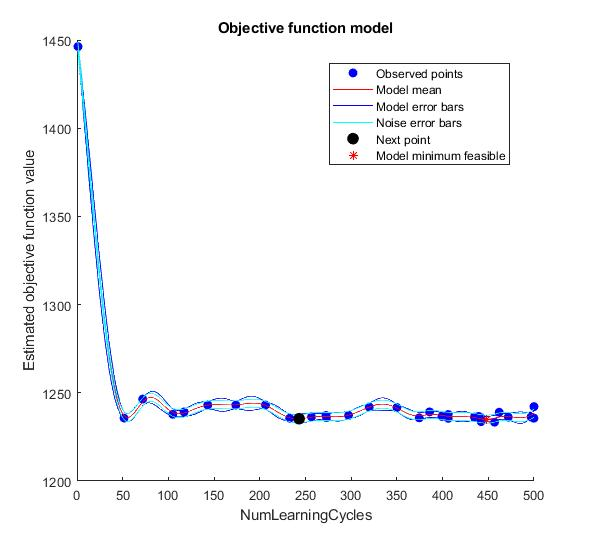
\includegraphics[height=6cm]{img/RFNumLearCyclesVMinMRSE}
\caption{RF Number of Learners versus RMSE}
\end{figure}

From the above graph you can see that there is not much difference between using 50 trees and 500. We have kept it at 499 as the results against the test set were better (if we cared about computational efficiency, we might cap at around 50 trees).
Using K-Fold validation on Random Forest made the results worse.

\section{Implementation Details}
For the implementation of the top models, we chose to use a single script named main to hold the majority of the code. This was to enable the easy running of all sections of code at once. This was also so that it was straightforward to run all of the code from top to bottom and reset all variables so that previous runs couldn't pollute the next run. By setting the data transformations to run each time the code ran we could ensure that our dataset remained pure and allowed for experimentation (such as how changing the hybrid's MPG from 202 to different numbers affected the models (it made the linear regression better and random forest worse)).

We used the rng function to set the random number seed so that all of the results were reproducible (this has the risk of the models being trapped in local minimums rather than finding the best parameters). Using the seed of 42 rather than 52 gave an RMSE of 1799.16 for Linear Regression (versus 1818.02) and 1115.55 for Random Forest (versus 1177.40). So, there is a much bigger effect on Random Forest, but not much difference for Linear Regression (either way Random Forest performed much better than Linear Regression).

For both models we excluded the tax and transmission type columns. For tax it was because it is derived from other columns and for transmission type it is because it had little effect on the price column.

For linear regression we normalised the training data and then normalised the test data using the same parameters. This dramatically increased the accuracy of the model (the RMSE went from £4782 down to £2428).

Using the script OptimizeLinearRegression we got the generalised hyperparameters for linear regression, then we used Bayesian optimisation to get a better lambda figure.

For random forest we used the function fitrensemble to train a collection of decision trees (we used a template tree so that we could adjust the minimum leaf size). We then used the script OptimiseRandomForest to find the best hyperparameters for the model. Then within the same script we used Bayesian optimisation to get the optimum number of trees.

To fairly analyse both models (so both were looked at the same way) we used the function analyseRegression, this worked out the MAE, RMSE and 1 - NMSE, then ran off the residual plots and other graphs.

To allow for some experimentation the code in main was sectioned so that the models could be run without needing to rerun the statistics and preparation sections. Long-running sections, such as Feature Importance, experiments with K Fold for Linear Regression and Random Forest and optimising the two models, were placed into their own code files and run once the main script had run.
So that we could get summary statistics on the data we created the function GetSummaryStats, this was to recreate Python's Pandas describe function in MATLAB. 


\bibliographystyle{plainnat}
\bibliography{MyLibrary}

\end{document}